        \documentclass{standalone}
        \usepackage{tikz}
        \begin{document}
        \fontsize{16px}{16px}\selectfont
        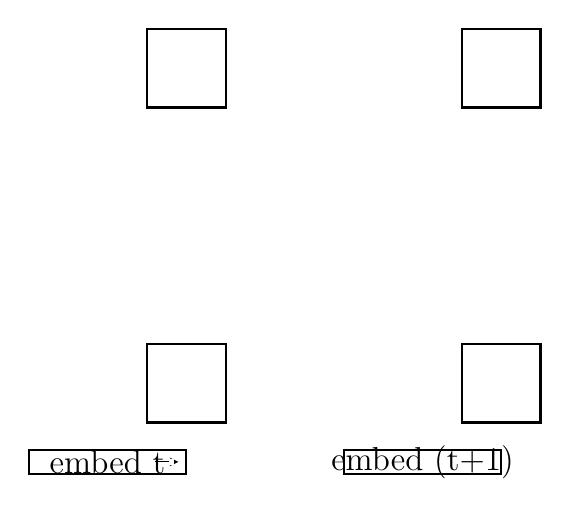
\begin{tikzpicture}

  \node (bx1) at (0,0) [draw,thick,minimum width=2cm,minimum height=0.3cm] {};
  \node[align=center,font=\large,rotate=0] at (bx1.center) {embed t};

  \node (bx2) at (4,0) [draw,thick,minimum width=2cm,minimum height=0.3cm] {};
  \node[align=center,font=\large,rotate=0] at (bx2.center) {embed (t+1)};

  \node (bx3) at (1,1) [draw,thick,minimum width=1cm,minimum height=1cm] {};
  \node (bx4) at (5,1) [draw,thick,minimum width=1cm,minimum height=1cm] {};
  \node (bx5) at (1,5) [draw,thick,minimum width=1cm,minimum height=1cm] {};
  \node (bx6) at (5,5) [draw,thick,minimum width=1cm,minimum height=1cm] {};

  \draw [->,>=stealth] (0.6,0) -- node[pos=.7,fill=white,inner sep=1pt]{}(0.9,0);
        \end{tikzpicture}
        \end{document}
